\chapter{一重項状態、ベルの不等式、そして複製不可能定理}

\lectureoverview{相対的な負符号が、単に相関した二スピン状態を回転不変な一重項状態に変える。その状態を全スピンを計算することによって同定し、その完全な反相関を用いてベル実験を定式化し、古典的命題を量子射影演算子に翻訳する。得られる確率はベルの古典的計数不等式に違反する。局所性、実験のタイミング、不確定性に関する問いは、次に線形量子力学の第二の帰結へと導く。すなわち、未知の状態は普遍的な複製機械によって複製することができない。}

\section{符号はどのような違いを生むのか}

二つの電子を考え、基底状態においてテンソル積の記号を省略する：
\begin{equation}
  \ket{ud}\equiv\ket{u}_1\otimes\ket{d}_2,
  \qquad
  \ket{du}\equiv\ket{d}_1\otimes\ket{u}_2.
\end{equation}
特に単純な二つの重ね合わせは一つの符号だけが異なる。
\begin{equation}
  \ket{\psi_\pm}
  =
  \frac{\ket{ud}\pm\ket{du}}{\sqrt2}.
  \label{eq:l05-two-signs}
\end{equation}
因子\(1/\sqrt2\)により全確率が1になる。どちらの状態でも、第三軸に沿った測定は反対の答えを与える。すなわち、電子1が上向きなら電子2は下向きであり、その逆も成り立つ。したがって、その相関だけからは符号を検出できない。それにもかかわらず、二つの状態は物理的に異なる。

計算ではパウリ作用を繰り返し用いる。
\begin{align}
  \sigma_1\ket{u}&=\ket{d},&
  \sigma_1\ket{d}&=\ket{u},\nonumber\\
  \sigma_2\ket{u}&=i\ket{d},&
  \sigma_2\ket{d}&=-i\ket{u},\nonumber\\
  \sigma_3\ket{u}&=\ket{u},&
  \sigma_3\ket{d}&=-\ket{d}.
  \label{eq:l05-pauli-actions}
\end{align}
電子1に作用する演算子には\(\sigma_i\)を割り当て、電子2に作用する同一の族\(\tau_i\)を導入する。

\begin{figure}[htbp]
\centering
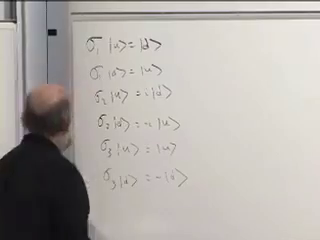
\includegraphics[width=0.62\linewidth]{lecture_05_figure_02.png}
\caption{比較全体で用いる完全なパウリ作用表。}
\lectureframe{00:03:15}
\end{figure}

どちらの状態でも、構成するスピンのいずれにも優先方向はない。
\begin{equation}
  \expect{\sigma_i}_{\psi_\pm}=0,
  \qquad
  \expect{\tau_i}_{\psi_\pm}=0,
  \qquad i=1,2,3.
  \label{eq:l05-local-zero}
\end{equation}
例えば、プラス状態について要求された明示的な確認を行うと、
\begin{align}
  \bra{\psi_+}\sigma_3\ket{\psi_+}
  &=
  \frac12
  \bigl(\bra{ud}+\bra{du}\bigr)
  \bigl(\ket{ud}-\ket{du}\bigr)\nonumber\\
  &=
  \frac12(1-1)=0.
  \label{eq:l05-sigma3-expectation}
\end{align}
交差項は\(\braket{ud}{du}=0\)であるため消える。

\begin{figure}[htbp]
\centering
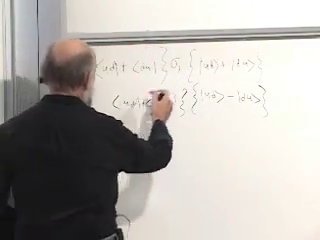
\includegraphics[width=0.78\linewidth]{lecture_05_figure_03.png}
\caption{プラス状態の期待値は、\(\sigma_3\)を作用させ、直交性を用いることによって評価される。}
\lectureframe{00:07:00}
\end{figure}

\begin{classroomqa}
\lecturetimestamp{00:07:13}
\audiencequestion{期待値がゼロであることは、単一のスピンが値ゼロを持つと測定できることを意味するのか。}
\lecturerresponse{いいえ。一つのスピンの成分は\(+1\)と\(-1\)という結果しか持たず、\(\sigma_i\)はゼロ固有値を持たない。式~\eqref{eq:l05-local-zero}が述べているのは、繰り返し測定が公平なコイントスであるということであり、個々の結果がゼロであるということではない。}
\end{classroomqa}

したがって、最初のもっともらしい診断は失敗した。局所的な平均では相対符号を見ることができないので、対の性質を測定しなければならない。

\section{全スピンが一重項状態を選び出す}

対の磁気モーメントはベクトル和で表される。
\begin{equation}
  \boldsymbol{\Sigma}
  =
  \boldsymbol{\sigma}+\boldsymbol{\tau}.
\end{equation}
その第三成分は両方の基底ベクトルを消す。
\begin{align}
  (\sigma_3+\tau_3)\ket{ud}
  &=(1-1)\ket{ud}=0,\nonumber\\
  (\sigma_3+\tau_3)\ket{du}
  &=(-1+1)\ket{du}=0.
\end{align}
したがって、
\begin{equation}
  (\sigma_3+\tau_3)\ket{\psi_\pm}=0.
\end{equation}
どちらの符号の選択でも、全第三成分はすべての試行でゼロである。

第一成分がそれらを区別する。式~\eqref{eq:l05-pauli-actions}より、
\begin{align}
  (\sigma_1+\tau_1)\ket{ud}
  &=\ket{dd}+\ket{uu},\nonumber\\
  (\sigma_1+\tau_1)\ket{du}
  &=\ket{uu}+\ket{dd}.
\end{align}
したがって
\begin{align}
  (\sigma_1+\tau_1)\ket{\psi_+}
  &=
  \sqrt2\bigl(\ket{uu}+\ket{dd}\bigr),\nonumber\\
  (\sigma_1+\tau_1)\ket{\psi_-}
  &=0.
  \label{eq:l05-total-x}
\end{align}
プラス状態はこの観測量について期待値ゼロを持ちうるが、そのゼロ固有値固有状態ではない。

\begin{classroomqa}
\lecturetimestamp{00:13:02}
\audiencequestion{状態が消されないとき、全成分はどのような結果を持ちうるか。}
\lecturerresponse{各構成要素の答えは\(+1\)または\(-1\)であるから、その和は\(2\)、\(0\)、または\(-2\)でありうる。期待値がゼロであることは、毎回ゼロであることを強制しない。}
\end{classroomqa}

第二成分がテストを完成させる。その\(i\)の因子は反対称結合で相殺する。
\begin{equation}
  (\sigma_2+\tau_2)\ket{\psi_-}=0.
\end{equation}
したがって三つの成分すべてがマイナス状態を消す。
\begin{equation}
  \bigl(\boldsymbol{\sigma}+\boldsymbol{\tau}\bigr)
  \cdot\hat n\,\ket{\psi_-}=0
  \qquad\text{for every unit vector }\hat n.
  \label{eq:l05-singlet-any-axis}
\end{equation}

\begin{figure}[htbp]
\centering
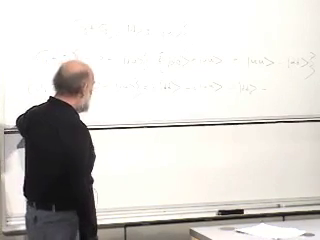
\includegraphics[width=0.84\linewidth]{lecture_05_figure_06.png}
\caption{マイナス状態を全スピンゼロとして同定する成分ごとの相殺。}
\lectureframe{00:16:30}
\end{figure}

反対称状態\(\ket{\psi_-}\)は\emph{一重項状態}である。それは回転不変である。すなわち、どの軸でも同じ全スピンの答え、ゼロを与える。式~\eqref{eq:l05-two-signs}の対称状態は三重項の部門に属する。

\begin{classroomqa}
\lecturetimestamp{00:19:06}
\audiencequestion{反対スピンの結果は平均でのみ成り立つのか。}
\lecturerresponse{一重項状態では、それはすべての試行で成り立つ。式~\eqref{eq:l05-singlet-any-axis}は固有ベクトル方程式であるから、両方の粒子で同じ成分を測定すると、常に和が固有値ゼロとなる答えが得られる。}
\end{classroomqa}

\begin{classroomqa}
\lecturetimestamp{00:19:36}
\audiencequestion{なぜもう一方の状態は三重項と呼ばれるのか。}
\lecturerresponse{その名前は全スピン1の多重項における三つの状態に由来する。その導出は後回しにする。現在の計算では、対称状態と一次元の一重項部門との対比だけが必要である。}
\end{classroomqa}

ボブが自分の電子の任意の成分を測定すれば、アリスが自分の電子の同じ成分を測定して得るであろう結果を直ちに知る。彼女の答えは反対でなければならない。これはアインシュタイン--ポドルスキー--ローゼンの相関である。隠れた硬貨の対も反対の結果を運ぶことができるが、それはあらかじめ取り決めた一つの質問に対してのみである。一重項は、どの空間軸が選ばれても完全な反相関を与える。

\begin{classroomqa}
\lecturetimestamp{00:20:55}
\audiencequestion{アインシュタイン、ポドルスキー、ローゼンが最初にもつれを発見したのか。}
\lecturerresponse{いいえ。シュレーディンガーがこの現象を論じ、もつれという言葉を導入した。EPRの議論は遠隔相関の問題を特に鮮明にした。}
\end{classroomqa}

\begin{classroomqa}
\lecturetimestamp{00:23:50}
\audiencequestion{即時の相関は因果性に反するのか、またどちらの観測者が先に測定するかは重要か。}
\lecturerresponse{利用可能なメッセージは伝達されない。アリスの局所的な結果は、ボブが測定するか否か、どの慣性系の順序でも、五十パーセントずつのままである。彼女が相関を検証できるのは、通常の古典的チャネルを通じてボブの結果を受け取った後だけであり、それは光より速く進むことはできない。}
\end{classroomqa}

\section{ベルの不等式は古典的な数え上げである}

ベルの結果の位置づけは不安定に感じられることがある。ある日には量子力学の最も深い特徴のように見え、別の日には形式体系のもう一つの不可避な帰結のように見える。ベル自身もファインマンも、両方の態度を表明することができた。しかし不等式は初等的である。驚きはその破れにある。

普通の対象の集合を考える。各対象は三つの性質\(A\)、\(B\)、\(C\)をもつかもたないかのいずれかである。\(N(A,\neg B)\)を、\(A\)をもつが\(B\)をもたないものの数とする。古典的な集合論理は次を意味する。
\begin{equation}
  N(A,\neg B)+N(B,\neg C)
  \geq
  N(A,\neg C).
  \label{eq:l05-bell-count}
\end{equation}
証明は集合の包含関係
\begin{equation}
  A\cap C^{c}
  \subseteq
  (A\cap B^{c})\cup(B\cap C^{c}).
  \label{eq:l05-set-inclusion}
\end{equation}
である。実際、\(A\cap C^c\)の要素は\(B\)に属するか属さないかのいずれかである。前者の場合それは\(B\cap C^c\)に属し、後者の場合それは\(A\cap B^c\)に属する。和集合を数えれば左辺の集合を過大に数えることしかできない。

\begin{figure}[htbp]
\centering
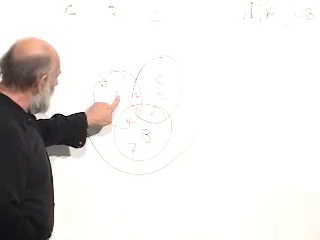
\includegraphics[width=0.78\linewidth]{lecture_05_figure_07.png}
\caption{盤面による証明は、三つの重なり合う古典的部分集合を非負の領域に分割する。}
\lectureframe{00:31:15}
\end{figure}

同値な言い方をすれば、三集合図の互いに素な領域を非負整数\(N_i\)でラベル付けする。式~\eqref{eq:l05-bell-count}の両辺は\(A\cap C^c\)に必要な領域を含み、左辺はさらに追加の非負領域を含む。量子的なものは何も入っていない。これは部分集合と通常の論理的選択肢に関する定理である。

\section{集合の言明をスピン実験に変える}

一重項状態にある多数の独立な電子対を用意し、電子1について三つの命題を定義する。
\begin{align}
  A&:\ \text{spin 1 is up at }0^\circ\text{, along the third axis},\nonumber\\
  B&:\ \text{spin 1 is up at }45^\circ\text{ in the }zx\text{-plane},\nonumber\\
  C&:\ \text{spin 1 is up at }90^\circ\text{, along the first axis}.
  \label{eq:l05-abc}
\end{align}

\begin{figure}[htbp]
\centering
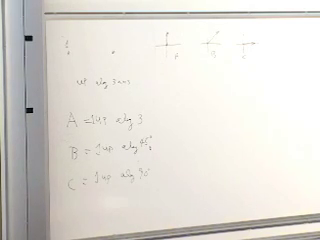
\includegraphics[width=0.82\linewidth]{lecture_05_figure_08.png}
\caption{三つのスピンの命題は一つの平面内の\(0^\circ\)、\(45^\circ\)、\(90^\circ\)に固定される。}
\lectureframe{00:39:00}
\end{figure}

一重項では、電子1についての命題の否定は、電子2についての肯定的な命題として書き換えられる。例えば、
\begin{align}
  \neg B
  &:\ \text{spin 1 is down at }45^\circ\nonumber\\
  &\Longleftrightarrow
  \text{spin 2 is up at }45^\circ.
\end{align}
同様に、\(\neg C\)は電子2が\(90^\circ\)で上向きであるという言明になる。

\begin{classroomqa}
\lecturetimestamp{00:40:04}
\audiencequestion{\(\neg C\)は電子2を\(90^\circ\)で下向きにすべきか。}
\lecturerresponse{いいえ。まず\(C\)を否定する。電子1は\(90^\circ\)で下向きである。完全な一重項の反相関により、電子2は同じ軸に沿って上向きになる。二つの反転は別々に保たなければならない。}
\end{classroomqa}

大きな集団では、数と確率は用意した対の共通の数だけしか違わない。回転不変性からも次が成り立つ。
\begin{equation}
  P(A,\neg B)=P(B,\neg C),
\end{equation}
なぜなら第二の実験は第一の実験を\(45^\circ\)だけ回転したものだからである。したがってベルの古典的不等式は次を要求するであろう。
\begin{equation}
  2P(A,\neg B)\geq P(A,\neg C).
  \label{eq:l05-bell-probability}
\end{equation}
ここでこれらの確率を計算する効率的な方法が必要である。

\section{命題は射影演算子になる}

通常の三次元ベクトル空間では、射影演算子は選ばれた部分空間に垂直なすべての成分を取り除く。一次元の射影演算子はベクトルを直交的に直線へ落とし、二次元の射影演算子はそれを平面へ落とす。\(P\)が指定された部分空間への射影であるならば、
\begin{equation}
  P\ket{\alpha}=\ket{\alpha_P}.
\end{equation}

\begin{figure}[htbp]
\centering
\includegraphics[width=0.76\linewidth]{lecture_05_figure_04.png}
\caption{幾何学的な射影とその演算子表記が並行して展開される。}
\lectureframe{00:49:53}
\end{figure}

\begin{figure}[htbp]
\centering
\begin{tikzpicture}[scale=1.05,>=Latex]
  \draw[->] (-0.25,0)--(4.0,0);
  \draw[thick] (-0.25,-0.25)--(3.55,2.6);
  \draw[->,very thick] (0,0)--(2.25,3.05)
    node[above] {\(\ket{\alpha}\)};
  \coordinate (P) at (2.72,1.98);
  \draw[dashed] (2.25,3.05)--(P);
  \draw[->,very thick] (0,0)--(P)
    node[right] {\(\ket{\alpha_P}\)};
  \node[below right] at (3.1,2.25) {projected subspace};
\end{tikzpicture}
\caption{射影幾何の明快な再構成。}
\end{figure}

一スピンのヒルベルト空間では、\(\sigma_3=+1\)という命題は\(\ket{u}\)が張る一次元部分空間に対応する。その射影演算子は次のように作用する。
\begin{equation}
  P_{\sigma_3=+1}
  \begin{pmatrix}\alpha\\\beta\end{pmatrix}
  =
  \begin{pmatrix}\alpha\\0\end{pmatrix},
  \qquad
  P_{\sigma_3=-1}
  \begin{pmatrix}\alpha\\\beta\end{pmatrix}
  =
  \begin{pmatrix}0\\\beta\end{pmatrix}.
  \label{eq:l05-projector-actions}
\end{equation}

\begin{classroomqa}
\lecturetimestamp{00:49:55}
\audiencequestion{最初の射影演算子は、ベクトルが垂直軸上でどれだけ高く達するかを報告するのか。}
\lecturerresponse{いいえ。それは直交する係数\(\beta\)を単に捨て去るだけである。成分はヒルベルト空間の振幅であり、スピンの通常の空間座標ではない。}
\end{classroomqa}

\begin{figure}[htbp]
\centering
\includegraphics[width=0.78\linewidth]{lecture_05_figure_05.png}
\caption{射影演算子はまず一般のスピノルに作用し、その後、明示的な行列として書かれる。}
\lectureframe{00:51:40}
\end{figure}

行列形式は
\begin{equation}
  P_{\sigma_3=+1}
  =
  \begin{pmatrix}1&0\\0&0\end{pmatrix}
  =
  \frac{I+\sigma_3}{2}.
  \label{eq:l05-p3}
\end{equation}
同じ構成は任意の単位ベクトル\(\hat n\)に沿っても成り立つ：
\begin{equation}
  P_{\boldsymbol{\sigma}\cdot\hat n=+1}
  =
  \frac{I+\boldsymbol{\sigma}\cdot\hat n}{2}.
  \label{eq:l05-pn}
\end{equation}

\begin{classroomqa}
\lecturetimestamp{00:53:09}
\audiencequestion{\(\sigma_1=+1\)への射影演算子は何か。}
\lecturerresponse{式~\eqref{eq:l05-p3}において\(\sigma_3\)を\(\sigma_1\)で置き換えると、\(P_{\sigma_1=+1}=(I+\sigma_1)/2\)となる。}
\end{classroomqa}

ボルンの規則は今や有用な命題の形をとる：
\begin{equation}
  P(\mathcal A\text{ is true in }\ket{\psi})
  =
  \bra{\psi}P_{\mathcal A}\ket{\psi}.
  \label{eq:l05-projector-born}
\end{equation}
規格化されたスピノル\(\ket{\psi}=(\alpha,\beta)^T\)に対して、\(P_{\sigma_3=+1}\)を伴う式~\eqref{eq:l05-projector-born}は\(|\alpha|^2\)を与える。まさにそうなるべきである。

この言葉遣いは、古典的命題と量子的命題の違いを明らかにする。古典論理では、性質は集合の部分集合に対応する。量子力学では、性質はヒルベルト空間の部分空間、あるいは同等にその射影演算子に対応する。部分集合とベクトル部分空間は同じ束演算に従わない。ベルの矛盾はその違いから生じる。

\subsection{結合ベル射影演算子}

\(A\wedge\neg B\)に対して、電子1は第三軸に沿って上でなければならず、電子2は
\begin{equation}
  \hat n_{45}=\frac{\hat x+\hat z}{\sqrt2}.
\end{equation}
に沿って上でなければならない。第二のスピンの関連する成分は
\begin{equation}
  \boldsymbol{\tau}\cdot\hat n_{45}
  =
  \frac{\tau_1+\tau_3}{\sqrt2}.
\end{equation}
したがって結合射影演算子は
\begin{equation}
  P_{A\wedge\neg B}
  =
  \frac{I+\sigma_3}{2}
  \frac{I+(\tau_1+\tau_3)/\sqrt2}{2}.
  \label{eq:l05-joint-projector}
\end{equation}

\begin{classroomqa}
\lecturetimestamp{00:59:18}
\audiencequestion{なぜ\(45^\circ\)スピン成分に因子\(1/\sqrt2\)が現れるのか。}
\lecturerresponse{方向は単位ベクトルでなければならない。その第一軸と第三軸の成分はともに\(1/\sqrt2\)であるから、対応する観測量は\((\tau_1+\tau_3)/\sqrt2\)である。}
\end{classroomqa}

\begin{classroomqa}
\lecturetimestamp{01:00:52}
\audiencequestion{式全体\(I+\boldsymbol{\tau}\cdot\hat n_{45}\)が2で割られているのか。}
\lecturerresponse{はい。射影演算子は\(\bigl(I+\boldsymbol{\tau}\cdot\hat n_{45}\bigr)/2\)であり、因子\(1/2\)は分子全体に掛かる。}
\end{classroomqa}

式~\eqref{eq:l05-joint-projector}の二つの因子は異なるテンソル因子に作用し、可換である。両方をまず適用すると、電子1が下であるすべての成分が除去され、次に\(\hat n_{45}\)に沿って電子2が下である残りのすべての成分が除去される。

\section{量子数が不等式を逆転させる}


\begin{equation}
  \ket{\psi_s}
  =
  \frac{\ket{ud}-\ket{du}}{\sqrt2}
\end{equation}
が一重項を表すものとする。まず
\begin{equation}
  P(A,\neg B)
  =
  \bra{\psi_s}P_{A\wedge\neg B}\ket{\psi_s}.
\end{equation}
から始める。因子\((I+\sigma_3)/2\)は\(\ket{du}\)を消し、\(\ket{ud}/\sqrt2\)を残す。次に第二の因子は
\begin{align}
  \frac{I+(\tau_1+\tau_3)/\sqrt2}{2}\ket{ud}
  &\notag\\[-0.3em]
  &=
  \frac12
  \left[
    \ket{ud}
    +\frac{\ket{uu}-\ket{ud}}{\sqrt2}
  \right]\nonumber\\
  &=
  \frac12
  \Biggl[
    \left(1-\frac1{\sqrt2}\right)\ket{ud}
  \nonumber\\
  &\qquad
    +\frac1{\sqrt2}\ket{uu}\Biggr].
  \label{eq:l05-projector-action}
\end{align}
を与える。\(\ket{uu}\)の項は一重項のブラとの重なりがゼロであり、生き残った規格化因子から
\begin{equation}
  P(A,\neg B)
  =
  \frac14\left(1-\frac1{\sqrt2}\right).
  \label{eq:l05-pab}
\end{equation}
が得られる。

\begin{figure}[htbp]
\centering
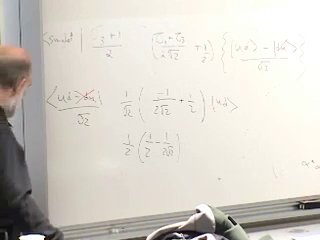
\includegraphics[width=0.88\linewidth]{lecture_05_figure_09.png}
\caption{射影演算子の計算は\(\ket{ud}\)の重なりを保ち、直交する\(\ket{uu}\)の寄与を捨て去る。}
\lectureframe{01:08:20}
\end{figure}

回転不変性により、次の方向の対についても同じ結果が得られる：
\begin{equation}
  P(B,\neg C)
  =
  \frac14\left(1-\frac1{\sqrt2}\right).
\end{equation}
\(A\wedge\neg C\)に対して、第二軸は第一空間軸であるから、
\begin{equation}
  P_{A\wedge\neg C}
  =
  \frac{I+\sigma_3}{2}\frac{I+\tau_1}{2}.
\end{equation}
第一の因子は再び\(\ket{ud}/\sqrt2\)を残す。\(\tau_1\)の項は\(\ket{uu}\)を生み、これは一重項のブラと直交するが、恒等演算子の項は生き残る。したがって
\begin{equation}
  P(A,\neg C)=\frac14.
  \label{eq:l05-pac}
\end{equation}
三つの結果を組み合わせると、
\begin{equation}
  \underbrace{
  P(A,\neg B)+P(B,\neg C)
  }_{\frac12(1-1/\sqrt2)\approx0.146}
  <
  \underbrace{
  P(A,\neg C)
  }_{\frac14=0.25}.
  \label{eq:l05-bell-violation}
\end{equation}

\begin{figure}[htbp]
\centering
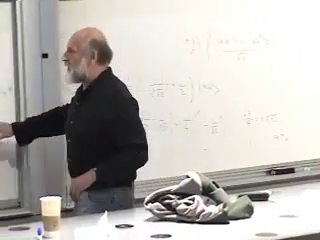
\includegraphics[width=0.84\linewidth]{lecture_05_figure_10.png}
\caption{完成した黒板の計算は、より小さいベルの左辺とより大きい右辺を示している。}
\lectureframe{01:12:15}
\end{figure}

式~\eqref{eq:l05-bell-violation}は式~\eqref{eq:l05-bell-probability}を逆転させる。結論は量子力学が自己矛盾をきたすということではない。一重項の相関は、三つのスピン命題すべてが遠方の測定の選択に依存しない通常の集合論的真理値をもつような局所古典模型から生じることはできない、ということである。古典的シミュレーションが相関を再現できるのは、少なくとも一つのベルの仮定、最も顕著には局所性を放棄することによってのみである。

\section{ベル実験が検証するもの}

量子力学はすでに破れを予言している。実験はさらに、一方の検出器がもう一方にどの設定または結果に出会ったかを知らせるという古典的な逃げ道を閉ざさなければならない。二つの翼は十分に離れており、選択と検出は時間的に十分近く、光速の信号がそれらの間を伝わることができないようにすべきである。アスペの実験は、そのタイミングと隔離を操作的に説得力のあるものにした。

\begin{classroomqa}
\lecturetimestamp{01:13:15}
\audiencequestion{量子力学がすでに答えを与えているなら、ベル実験は我々に何かを教えたのか。}
\lecturerresponse{それらは、まさにこの相関実験において自然が量子論の予言に従うかどうかを検証し、決定的なことに、二つの測定の翼を関連する光伝播時間において独立にした。実験的制御とタイミングそれ自体が大きな成果であった。}
\end{classroomqa}

\begin{classroomqa}
\lecturetimestamp{01:18:19}
\audiencequestion{アインシュタインが不気味な遠隔作用について論じた後、ベルは何を付け加えたか。}
\lecturerresponse{ベルは定量的な不等式を与えた。彼は、量子論的予測が局所的な古典的背後機構を排除する実行可能な相関実験を特定したのであり、異議を哲学的な不安の水準にとどめなかった。ベル自身は、これが不可避なのか深遠なのかについて曖昧な態度を保ち、標準的な量子力学に疑問を投げかけることにますます積極的になった。}
\end{classroomqa}

粒子は何マイルも離れていても一つの共同状態を共有しうるが、これは依然として小さな系に対する量子実験である。環境との相互作用は必要な位相関係を壊しやすい。空気分子、迷光光子、熱的擾乱が対ともつれ合いうるので、分離は冷たくよく隔離された環境で行わなければならない。

\begin{classroomqa}
\lecturetimestamp{01:19:53}
\audiencequestion{共通の状態が大きな距離に広がることは、これを巨視的な量子物体にするのか。}
\lecturerresponse{むしろ、遠く離れた小さな量子系と記述するのが適切である。その分離は大きくできるが、共同波動関数を保つことはますます微妙になる。環境との制御されない相互作用が有用なコヒーレンスを壊すからである。二つの普通のボウリング球は同じ実験を与えない。}
\end{classroomqa}

\begin{classroomqa}
\lecturetimestamp{01:21:23}
\audiencequestion{一方の粒子を測定すれば他方について相補的な情報が得られ、それによって不確定性原理を回避できるのか。}
\lecturerresponse{たとえば一方の粒子の位置を、他方の粒子の運動量を測定することができる。それは一つの粒子に対する非可換な観測量の同時測定ではない。単一系に対する不確定性の制限は回避されていない。}
\end{classroomqa}

\section{積はいつ「かつ」を意味するのか}

ベルの計算は二つの射影演算子を掛け合わせた。これは両立可能な命題に対してのみ論理積を表す。

\begin{classroomqa}
\lecturetimestamp{01:22:39}
\audiencequestion{なぜ二つの射影演算子の積が論理語「かつ」を表したのか。}
\lecturerresponse{二つの射影演算子が可換だからである。一方は電子1に作用し、他方は電子2に作用するので、その順序は無関係であり、両方の性質を一緒に検証できる。単一の電子に対しては、\((I+\sigma_3)/2\)と\((I+\sigma_1)/2\)は可換でなく、両方の軸に沿ったスピン上向きはこの種の共同で確定した命題ではない。}
\end{classroomqa}

ここも量子命題が通常の部分集合から逸脱する箇所である。古典的な共通部分は常に存在する。積射影演算子で表される量子的類似物は、関連する部分空間が両立可能なときにのみ意図された論理的意味を持つ。

同じ議論は測定そのものへも向かう。測定装置は指針状態を持つ。上向き電子が指針を一方へ動かし、下向き電子が他方へ動かすなら、重ね合わせの電子は二つの指針位置と もつれ合う。したがって測定は系と装置の間のもつれとして研究できる。その問題は、線形性のみを用いるより短い定理のために後回しにされる。

\begin{classroomqa}
\lecturetimestamp{01:25:09}
\audiencequestion{波動関数の収縮を、一つの測定が共同状態を制約することとして有用に捉えられるか。}
\lecturerresponse{その問いは測定過程に属する。装置と被測定系はもつれ合う。一方のスピン値は一方の指針位置と相関し、他方の値は他方と相関する。測定の詳細な議論は延期される。}
\end{classroomqa}

\section{線形性は万能ゼロックス機を禁じる}

時間発展について必要な事実はただ一つである。ある物理過程が
\begin{equation}
  \ket{a}\longrightarrow\ket{a'},
  \qquad
  \ket{b}\longrightarrow\ket{b'},
\end{equation}
を送るなら、線形性は
\begin{equation}
  \alpha\ket{a}+\beta\ket{b}
  \longrightarrow
  \alpha\ket{a'}+\beta\ket{b'}.
  \label{eq:l05-linearity}
\end{equation}
を要求する。

普通の複写機は古典情報を制御可能なほど小さな誤差で複製できる。量子論的要求はより強い。一つの固定された装置が、提示された任意の状態の完全な振幅を複製しなければならない。これが、ノークローニングが量子ゼロックス原理とも呼ばれる理由である。

一つの入力ポートと二つの出力ポートを持つ機械を想像せよ。それが第三軸基底をクローンするなら、
\begin{equation}
  \ket{u}\longrightarrow\ket{uu},
  \qquad
  \ket{d}\longrightarrow\ket{dd}.
  \label{eq:l05-clone-basis}
\end{equation}
を実行しなければならない。機械は出力にエネルギー、質量、電荷を供給できる。保存則の帳尻は障害ではない。矛盾は変換の状態依存性に関するものである。

\begin{figure}[H]
\centering
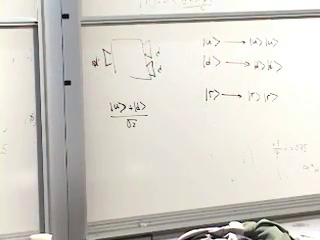
\includegraphics[width=0.86\linewidth]{lecture_05_figure_11.png}
\caption{仮想的な一入力二出力の機械は両方の基底状態を複製することを要求される。}
\lectureframe{01:33:45}
\end{figure}

ここで右を向いたスピン
\begin{equation}
  \ket{r}
  =
  \frac{\ket{u}+\ket{d}}{\sqrt2}.
  \label{eq:l05-right-state}
\end{equation}
を入力する。式~\eqref{eq:l05-linearity}と\eqref{eq:l05-clone-basis}は出力
\begin{equation}
  \ket{r}
  \longrightarrow
  \frac{\ket{uu}+\ket{dd}}{\sqrt2}.
  \label{eq:l05-linear-output}
\end{equation}
を強制する。一方、正確なクローニングは二つの独立なコピーを要求する。
\begin{align}
  \ket{rr}
  &=
  \ket{r}\otimes\ket{r}\nonumber\\
  &=
  \frac12
  \left(
    \ket{uu}+\ket{ud}+\ket{du}+\ket{dd}
  \right).
  \label{eq:l05-cloned-output}
\end{align}
式~\eqref{eq:l05-cloned-output}の混合項は式~\eqref{eq:l05-linear-output}には存在しない。二つの出力は異なる。

\begin{figure}[H]
\centering
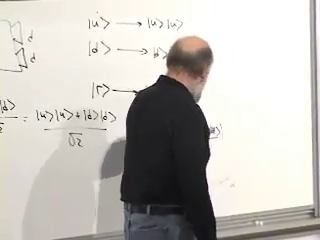
\includegraphics[width=0.72\linewidth]{lecture_05_figure_12.png}
\caption{線形性は平行スピンの項のみを生み出すが、真に右向きの2つのコピーは混合項も両方含む。}
\lectureframe{01:35:20}
\end{figure}

\begin{theorem}[No-cloning]
いかなる単一の物理的機械も、すべての未知の量子状態を正確に複製することはできない。
\end{theorem}

\begin{proof}
式~\eqref{eq:l05-clone-basis}のように、ある機械が直交基底状態を複製すると仮定する。すると線形性により、それらの重ね合わせに対する出力は式~\eqref{eq:l05-linear-output}に定まる。同じ入力を正確に複製することは式~\eqref{eq:l05-cloned-output}を要求する。2つの状態ベクトルは異なるため、仮定された万能機械は存在し得ない。
\end{proof}

その理由は構造的なものである。\(\ket{\psi}\) を \(\ket{\psi}\otimes\ket{\psi}\) へ移すことは振幅について二次であるのに対し、完全な量子状態の許されるあらゆる時間発展は線形である。

\begin{classroomqa}
\lecturetimestamp{01:35:49}
\audiencequestion{この証明は2つの出力が独立であると仮定しているのか。}
\lecturerresponse{はい、2つのコピーは独立に使用可能なコピーでなければならないからである。独立な系はテンソル積によって結合する。それゆえ右向きの2つのコピーは\(\ket{r}\otimes\ket{r}\)である。別々に使用できない相関した出力は2つのコピーではない。}
\end{classroomqa}

\begin{classroomqa}
\lecturetimestamp{01:37:20}
\audiencequestion{レーザーは誘導放出を通じて光子の状態を複製しているように見える。この議論はどこで破綻するのか。}
\lecturerresponse{原子と電磁モードも関与している。それらの状態は出力に寄与し、万能複製の観点からはノイズとして現れる。近似的複製は可能であるが、完全な状態非依存の複製は不可能である。}
\end{classroomqa}

\begin{classroomqa}
\lecturetimestamp{01:40:24}
\audiencequestion{量子情報は複製できなくても転送できるのか。}
\lecturerresponse{はい。転送は異なる操作である。すなわち、元の系が状態を保持する必要はない。複製不可能性が禁じるのは、2つの独立な完全コピーで終わることであり、状態をある担体から別の担体へ移すことではない。}
\end{classroomqa}

\begin{classroomqa}
\lecturetimestamp{01:41:03}
\audiencequestion{入力状態は未知でなければならないのか。}
\lecturerresponse{状態が事前に既知であれば、その状態にある系をさらに用意することも、選ばれた直交基底に適合する装置を構成することもできる。不可能なのは、任意の入力を受け取り、どの状態が到来したかを事前に知ることなくそれを複製する単一の機械である。}
\end{classroomqa}

\begin{classroomqa}
\lecturetimestamp{01:42:35}
\audiencequestion{右状態の2つの表式のうち、実際の機械の出力はどちらか。}
\lecturerresponse{線形性は式~\eqref{eq:l05-linear-output}を強制し、複製は式~\eqref{eq:l05-cloned-output}を要求する。それらの不一致こそがまさに矛盾である。}
\end{classroomqa}

\begin{classroomqa}
\lecturetimestamp{01:43:40}
\audiencequestion{もつれた2粒子状態が担う余分な情報は定量化できるのか。}
\lecturerresponse{1つのスピンの純粋状態は2つの実物理パラメータをもつ。別々に用意された2つのスピンは4つを与えるが、4次元の2スピンヒルベルト空間における一般の純粋状態は、規格化と全体位相を除いた後で6つをもつ。追加の状態にはもつれた状態が含まれ、そのもつれの度合いはもつれエントロピーによって定量化できる。}
\end{classroomqa}

\enlargethispage{4\baselineskip}
式~\eqref{eq:l05-two-signs}の符号は今や3つの役割を果たしてきた。それは唯一の全スピンゼロ状態を選び出し、古典的な集合不等式を破る相関を与え、線形な量子時間発展と2つのコピーを作る非線形な行為との違いを露わにした。それぞれの結果は、結合状態を既存の局所的な性質の一覧としてではなく、その完全なテンソル積空間におけるベクトルとして扱うことから生じる。
